\section{Design Architetturale}

\subsection{Architettura generale}
Per garantire una corretta separazione delle responsabilità fra componenti, il progetto adotta il pattern architetturale MVC. Come mostrato in Figura \ref{fig:mainarchitecture} la View permette di fornire in input il set di parametri necessario all'avvio di una simulazione al controller. Il Controller provvede quindi ad inizializzare la simulazione con i dati ricevuti in input e a metterla in moto.

\begin{figure}[h!]
\centering
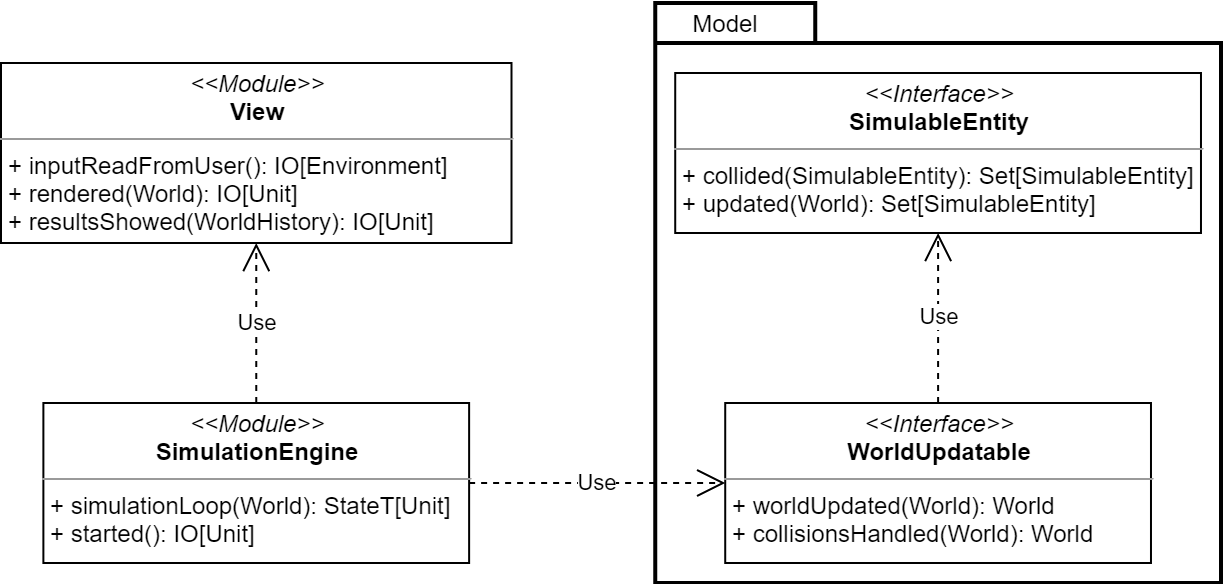
\includegraphics[width=\textwidth, scale=0.44]{img/MainArchitecture.png}
\caption{Design architettura principale}
\label{fig:mainarchitecture}
\end{figure}

\subsection{Pattern architetturali}